\section{URDAD's Meta Model \label{sec:metamodel}}

URDAD's meta model provides a formal description of URDAD's domain of discourse. It will be used to support the URDAD methodology of requirements specification. A meta model is a ``logical information model that specifies the modeling elements used within another (or the same) modeling notation'' \cite{_ieee_2003}. 

URDAD's meta model formalizes the modelling constructs needed for the specification of service requirements and the technology-neutral design of business processes which fulfil such requirements. It is specified in \emph{Ecore} which is an implementation of \emph{EMOF}. The \emph{Eclipse} modelling tool suite\cite{gronback_model_2008} supports the automatic generation of concrete textual and diagrammatic grammars, \emph{QVT}-based model transformations, as well as the integrated use of the Object Constraint Language (OCL) \cite{_object_2010}. An automatic translation of the meta model into a representation within the Web Ontology Language (OWL DL) ontology was done to facilitate automated satisfiability checking (see Section \ref{sec:assessment}).

Our meta model was designed to contain the smallest sufficient set of concepts that describe URDAD's service-oriented analysis and design specifications.  It was influenced by the UML and the Business Process Execution Language (BPEL) in the area of data structure and process specification. One of its underlying assumptions is the internal `statelessness' of services; `state' is assumed to be stored in the services' environments. The metamodel describes the notions of a responsibility domain, intra-model relationships facilitating traceability, service contracts including pre-conditions and their associated exceptions, post-conditions, as well as service-specific request and result classes. Our DSL also describes a system of parametrised, reusable operational constraints, which are applied to information obtained from the environment sourced through services.

Using tools like EMFText \cite{heidenreich_derivation_2009} one can either generate or specify a textual grammar for a metamodel, and from this grammar both a parser and a language-aware editor supporting syntax checking and auto-completion. In this section we illustrate core aspects of the URDAD DSL through an example encoded in the grammar which we have defined for the language. The textual grammar is meant to enable requirements specialists to specify URDAD DSL models within a simple and intuitive textual syntax. Ultimate,y we expect a graphical syntax to be still more accessible for requirements specialists than the textual syntax.

%--------------------------
\subsection{The Core of URDAD's Meta Model}

The core module (see Figure \ref{fig:coreModule}) introduces core concepts like the URDAD model itself, model elements, stake holders, responsibility domains, expressions and annotations.
\begin{figure*}[thb]
  \centering
  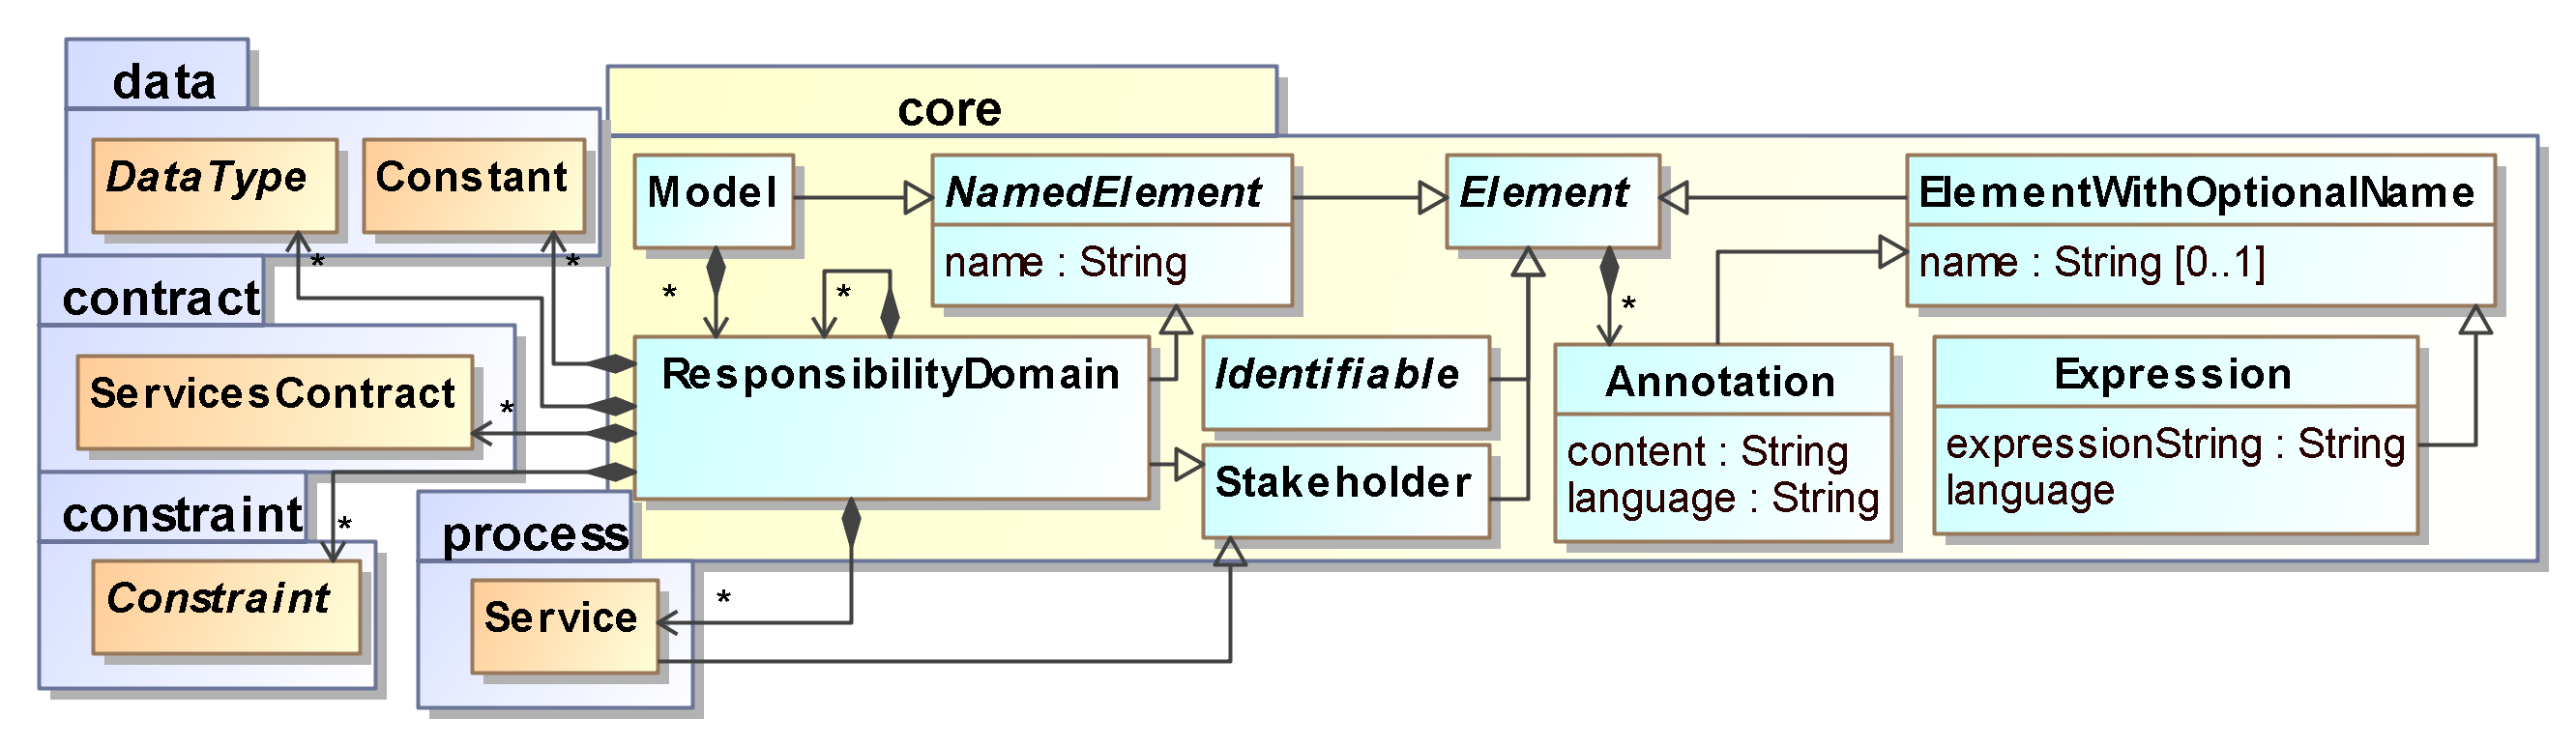
\includegraphics[width=\pagewidth]{core}\\   
  \caption{The core elements of URDAD}
  \label{fig:coreModule}
\end{figure*}

A responsibility domain covers a coherent unit of functionality at a particular level of granularity. Responsibility domains are meaningful groupings of service contracts. Thereby our notion of `responsibility domain' is similar to the notion of `unity criteria' in \cite{gonzalez_unity_2009}. Technically, responsibility domains are packaging constructs to subsume model elements under a unique name space. Note that they also define the boundaries between different levels of granularity. 

%-----------------------
\subsection{Constraints}

Constraints are required for the specification of functional requirements (pre- and post-conditions), data structure constraints and decision points in processes. The Object-Constraint Language (OCL) has become the de-facto standard for specifying constraints across object graphs. However, in a service-oriented approach and in the context of reusable, parametrised constraints the OCL alone is not expressive enough. 

Firstly, in a service-oriented context the actual environmental state is only accessible by using services which query the environment and not by traversing an object graph. The specification of constraints must thus relate to the specification of services through which information is sourced from the environment together with a set of data structure constraints on the obtained information. OCL can be used for the latter, but is insufficient for the complete specification of a constraint.

Secondly, the definition of reusable constraints requires support for binding parameters. \emph{For example}, assume a constraint that some `Person' must be `registered'. Such a constraint can contribute to pre- or post-conditions of services. Hence, to be able to do so, the person identifier would have to be passed as a parameter to the constraint entity. 

The following listing shows an extract of the textual representation of our `registration' example. It illustrates the specification of a simple parametrised constraint which includes the specification of a process that extracts information from the environment as well as a data constraint to be checked against the such-obtained information.
\lstset{language=urdad,caption=Specifying a state constraint in the textual URDAD DSL syntax.,label=constraintTextSyntax}
\begin{lstlisting}[numbers=left,escapechar=|]
StateConstraint studentEnrolledForPresentation receiving Variable enrollForPresentationRequest ofType EnrollForPresentationRequest
{
 stateAssessmentProcess doSequential
 {
  create Variable getEnrollmentsRequest ofType GetEnrollmentsRequest
  set Query OCL:"getEnrollmentsRequest.presentationIdentifier" equalTo Query OCL:"enrollForPresentationRequest.presentationIdentifier"
  requestService getEnrollments with getEnrollmentsRequest yielding Variable getEnrollmentsResult ofType GetEnrollmentsResult
 }
 Constraint OCL:"getEnrollmentsResult.enrollments.includes (enrollForPresentationRequest.personIdentifier)"
}
\end{lstlisting}

As depicted in Figure \ref{fig:constraintModule}, the constraints module provides the concept of re-usable constraints with standard logical operators to formulate complex constraint expressions.
\begin{figure*}[thbp]
  \centering
  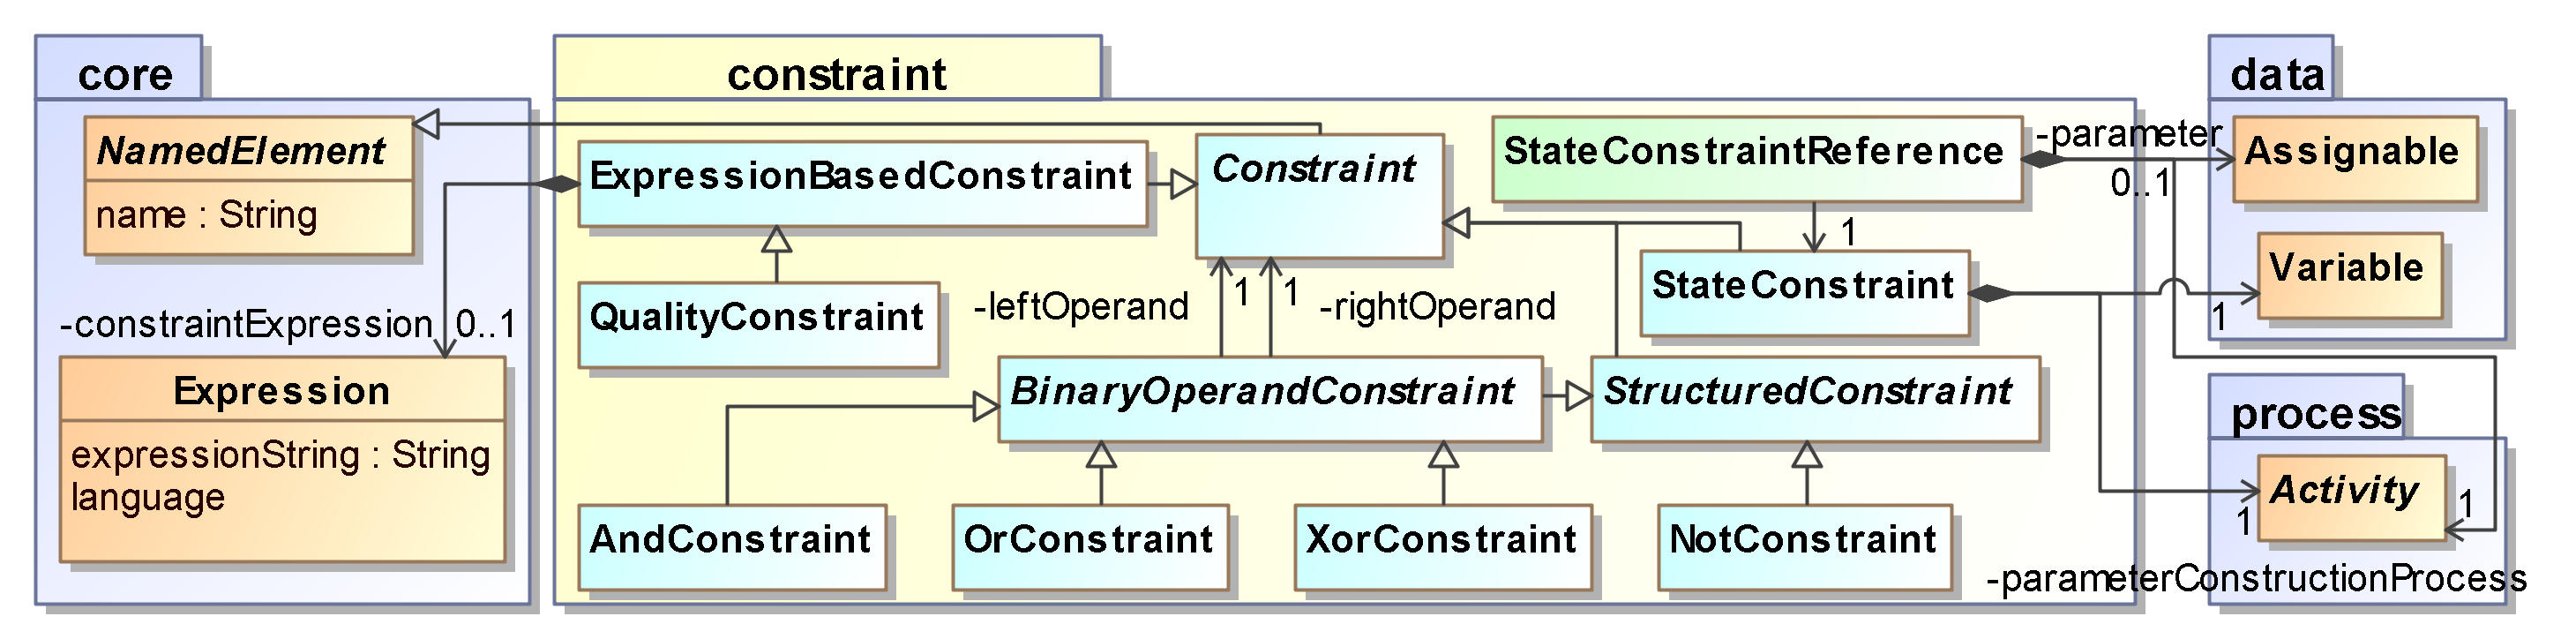
\includegraphics[width=\pagewidth]{constraint}\\   
  \caption{The constraint specification elements of URDAD}
  \label{fig:constraintModule}
\end{figure*}

%----------------------------
\subsection{Service Contracts}

A service contract comprises both functional and non-functional quality requirements. Every requirement is associated with a stakeholder which is either a responsibility domain or another service. Functional service requirements are expressed in terms of the above-mentioned pre- and post-conditions, together with exception rules for the case that any pre-condition is not fulfilled. 

A post-condition can specify either the computational output of a service, or its \emph{side effects} on its environment. Due to a service potentially creating a lasting change to its environment, the URDAD DSL allows the designation of inverse services through which these lasting effects can be reversed. Explicit post-conditions thus also help to specify such undo-services.

A service contract specifies a single service request object that contains information pertaining to the request and a single result object, which contains the information associated with the result of the executed service. The data structures for these request and result objects are service-specific and are not meant to be reused (though their components, which are domain objects, are most likely to be reused). 

Below we illustrate the specification of a service contract in our URDAD DSL grammar.
\lstset{language=urdad,caption=Specifying a service contract in the textual URDAD DSL syntax.,label=contractTextSyntax}
\begin{lstlisting}[numbers=left,escapechar=|]
ServiceContract enrollForPresentation
{
 FunctionalRequirements receiving Variable enrollForPresentationRequest ofType EnrollForPresentationRequest
 {
  PreCondition enrollmentPrerequisitesMet requiredBy (TrainingRegulator Student) raises EnrollmentPrerequisitesNotSatisfiedException checks constraint enrollmentPrerequisitesForPresentationMet with ValueOf enrollForPresentationRequest
  PostCondition enrollmentProcessPerformed requiredBy (Student Client TrainingRegulator) ensures constraint studentEnrolledForPresentation          with ValueOf studentEnrolledRequest constructedUsing doSequential
  {
   create Variable studentEnrolledRequest ofType StudentEnrolledRequest
   set Query OCL:"studentEnrolledRequest.personIdentifier" equalTo Query OCL:"enrollForPresentationRequest.personIdentifier"                            
   set Query OCL:"studentEnrolledRequest.presentationIdentifier" equalTo Query OCL:"enrollForPresentationRequest.presentationIdentifier"                            
  }  
  PostCondition invoiceIssued ...
 }            
 Request DataStructure EnrollForPresentationRequest 
 {
  has identification presentationIdentifier identifying Presentation
  has identification studentIdentifier identifying Person
  has identification clientIdentifier identifying LegalEntity         
 }
 Result DataStructure EnrollForPresentationResult 
 {
  has component proofOfEnrollment ofType ProofOfEnrollment
  has component invoice ofType Invoice
  has component studyGuide ofType StudyGuide
 }
}
\end{lstlisting}


Figure \ref{fig:contractModule} shows the URDAD DSL support for the specification of service contracts as packaged within a contract module.

\begin{figure*}[thbp]
  \centering
  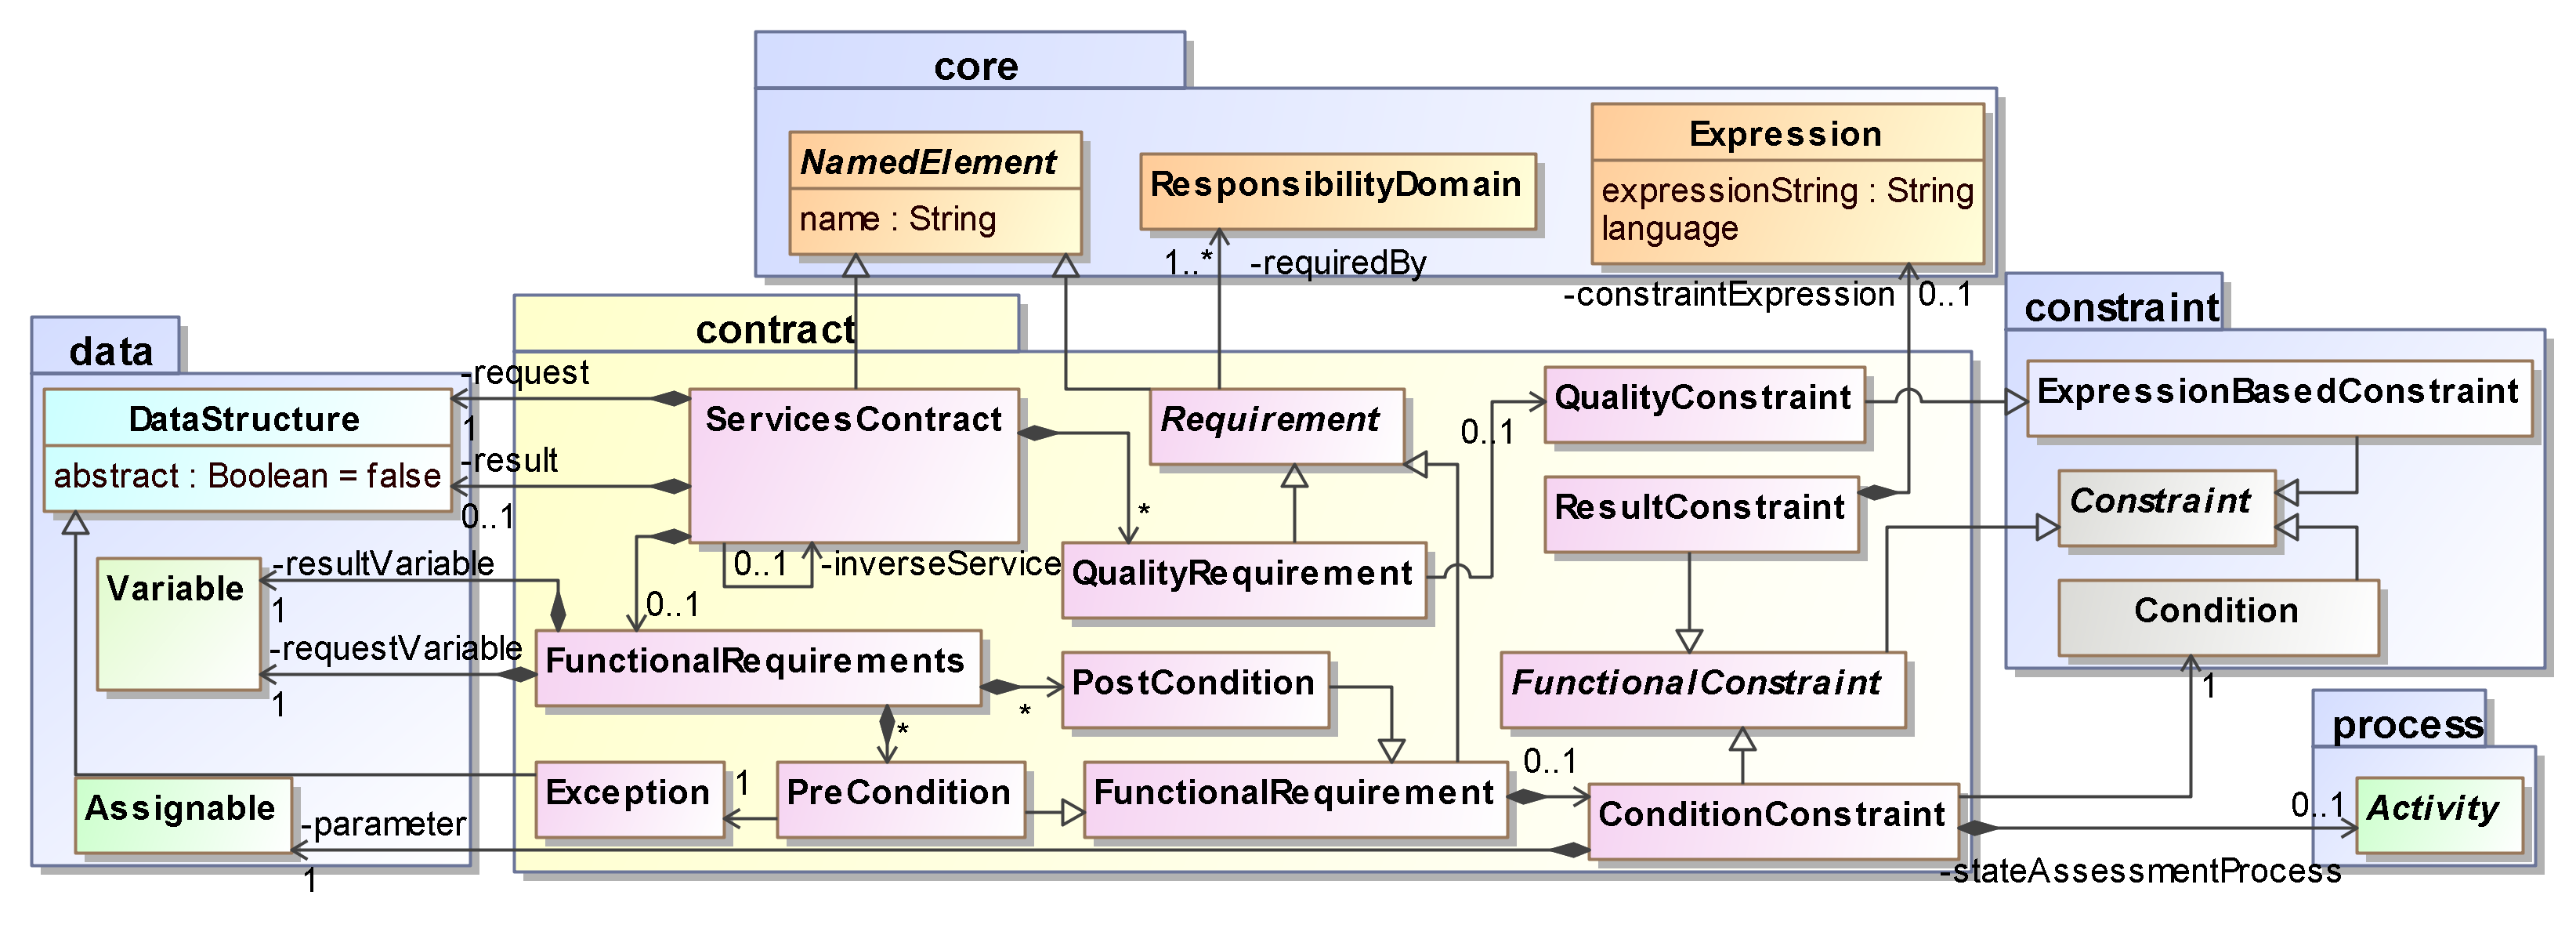
\includegraphics[width=\pagewidth]{contract}\\   
  \caption{The contract specification elements of URDAD}
  \label{fig:contractModule}
\end{figure*}


%--------------------------
\subsection{Data Structures}

The data module of the URDAD meta model is depicted in Figure \ref{fig:dataStructureModule}. It allows for an object-oriented approach to data structure specification which is directly aligned with UML class descriptions. In addition to the familiar type relationships - Association, Aggregation and Composition, URDAD DSL introduces a new, weaker type relationship called \emph{Identification}. This is conceptually similar to a strongly-typed \emph{Uniform Resource Identifier} (URI), in that it uniquely identifies objects within the model, but without implying an active message path to the object as UML \emph{Association}s do.
 
\begin{figure*}[thbp]
  \centering
  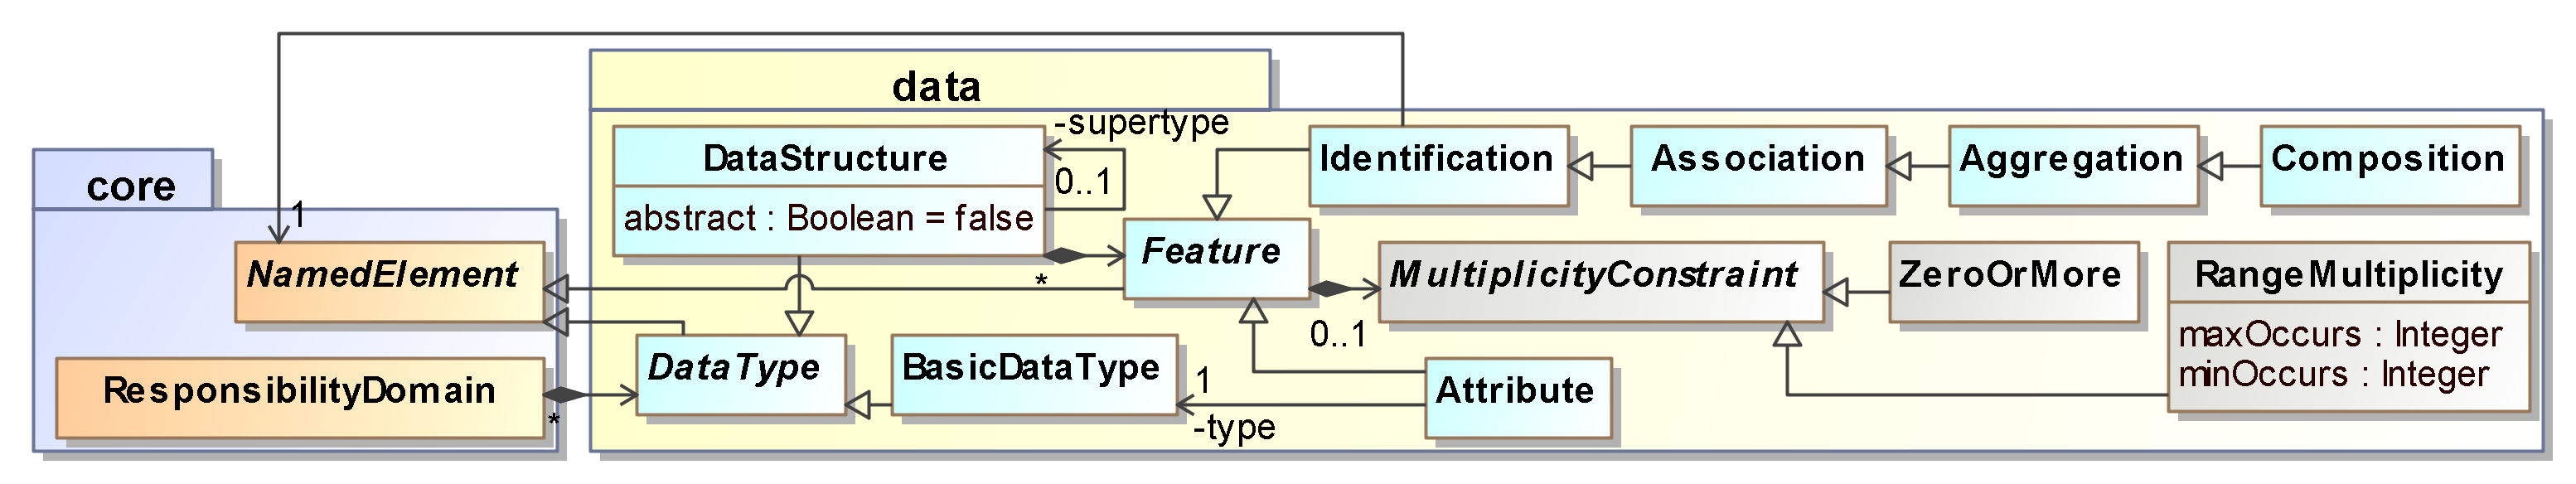
\includegraphics[width=\pagewidth]{data}\\   
  \caption{The data definition elements of URDAD}
  \label{fig:dataStructureModule}
\end{figure*}

%--------------------
\subsection{Processes}

The process package of the URDAD meta model describes the concept of a service as a concrete unit of functionality in fulfillment of its service contract. The responsibility allocation step of the URDAD methodology is supported by capturing the lower level service requirements for a service, relating each service used to either the assessment of a pre-condition or the realization of a post-condition. This is done via \verb+usedToAddress+ links representing satsifaction links as in  \cite{ramesh_toward_2001}). 

The second aspect of a service is the specification of a process which is assembled from service requests associated with the lower level service contracts used to address the functional requirements of the service. Note that decoupling of levels of granularity via service contracts is enforced. The URDAD metamodel assumes that the selection of concrete service providers for the lower level services is either done by the deployment environment through mechanisms like \emph{dependency injection} or specified during the implementation mapping phase.

The URDAD metamodel also contains explicit modelling constructs for creating and manipulating local process variables,  for handling an exception raised by a lower level service, for raising an exception associated with a pre-condition of the service, and for the return of a computational result. The following listing illustrates how a service contract is denoted in the grammar of our URDAD DSL.

\lstset{language=urdad,caption=Specifying a service in the textual URDAD DSL syntax.,label=serviceTextSyntax}
\begin{lstlisting}[numbers=left,escapechar=|]
Service enrollForPresentationImpl realizes enrollForPresentation receiving Variable enrollForPresentationRequest ofType EnrollForPresentationRequest
{
 use checkStudentSatisfiesEnrollmentPrerequisites toAddress (enrollmentPrerequisitesMet)
 use issueInvoice toAddress (financialPrerequisitesSatisfied invoiceIssued) 
 use performEnrollment toAddress (invoiceIssued)
   
 Process doSequential
 {
  create Variable checkStudentSatisfiesEnrollmentPrerequisitesRequest ofType CheckStudentSatisfiesEnrollmentPrerequisitesRequest               
  set Query OCL:"enrollForPresentationRequest.studentIdentifier" equalTo Query OCL:"checkEnrollmentPrerequisitesRequest.studentIdentifier"
  set Query OCL:"enrollForPresentationRequest.presentationIdentifier" equalTo Query OCL:"checkEnrollmentPrerequisitesRequest.presentationIdentifier"
                     
  requestService checkStudentSatisfiesEnrollmentPrerequisites with checkStudentSatisfiesEnrollmentPrerequisitesRequest yielding Variable checkStudentSatisfiesEnrollmentPrerequisitesResult ofType CheckStudentSatisfiesEnrollmentPrerequisitesResult
  choice
  {
   if Constraint enrollmentMeetsPrerequisitesMet OCL:"checkStudentSatisfiesEnrollmentPrerequisitesResult.enrollmentPrerequisitesMet = true" doSequential
   {
    ...
    requestService issueInvoice with issueInvoiceRequest yielding Variable issueInvoiceResult ofType IssueInvoiceResult
    {
     on FinancialPrerequisitesNotSatisfiedException raiseException FinancialPrerequisitesNotSatisfiedException
    }
    ...
    requestService performEnrollment with enrollRequest yielding Variable performEnrollmentResult ofType PerformEnrollmentResult
          
    create Variable enrollForPresentationResult ofType EnrollForPresentationResult
    set Query OCL:"issueInvoiceResult.invoice" equalTo Query OCL:"enrollForPresentationResult.invoice"
    ...                       
    returnResult  enrollForPresentationResult
   }
   else raiseException EnrollmentPrerequisitesNotSatisfiedException
  }
 }
}                 
\end{lstlisting}

Figure \ref{fig:processModule} shows the pocess modules of the URDAD meta model.
\begin{figure*}[thbp]
  \centering
  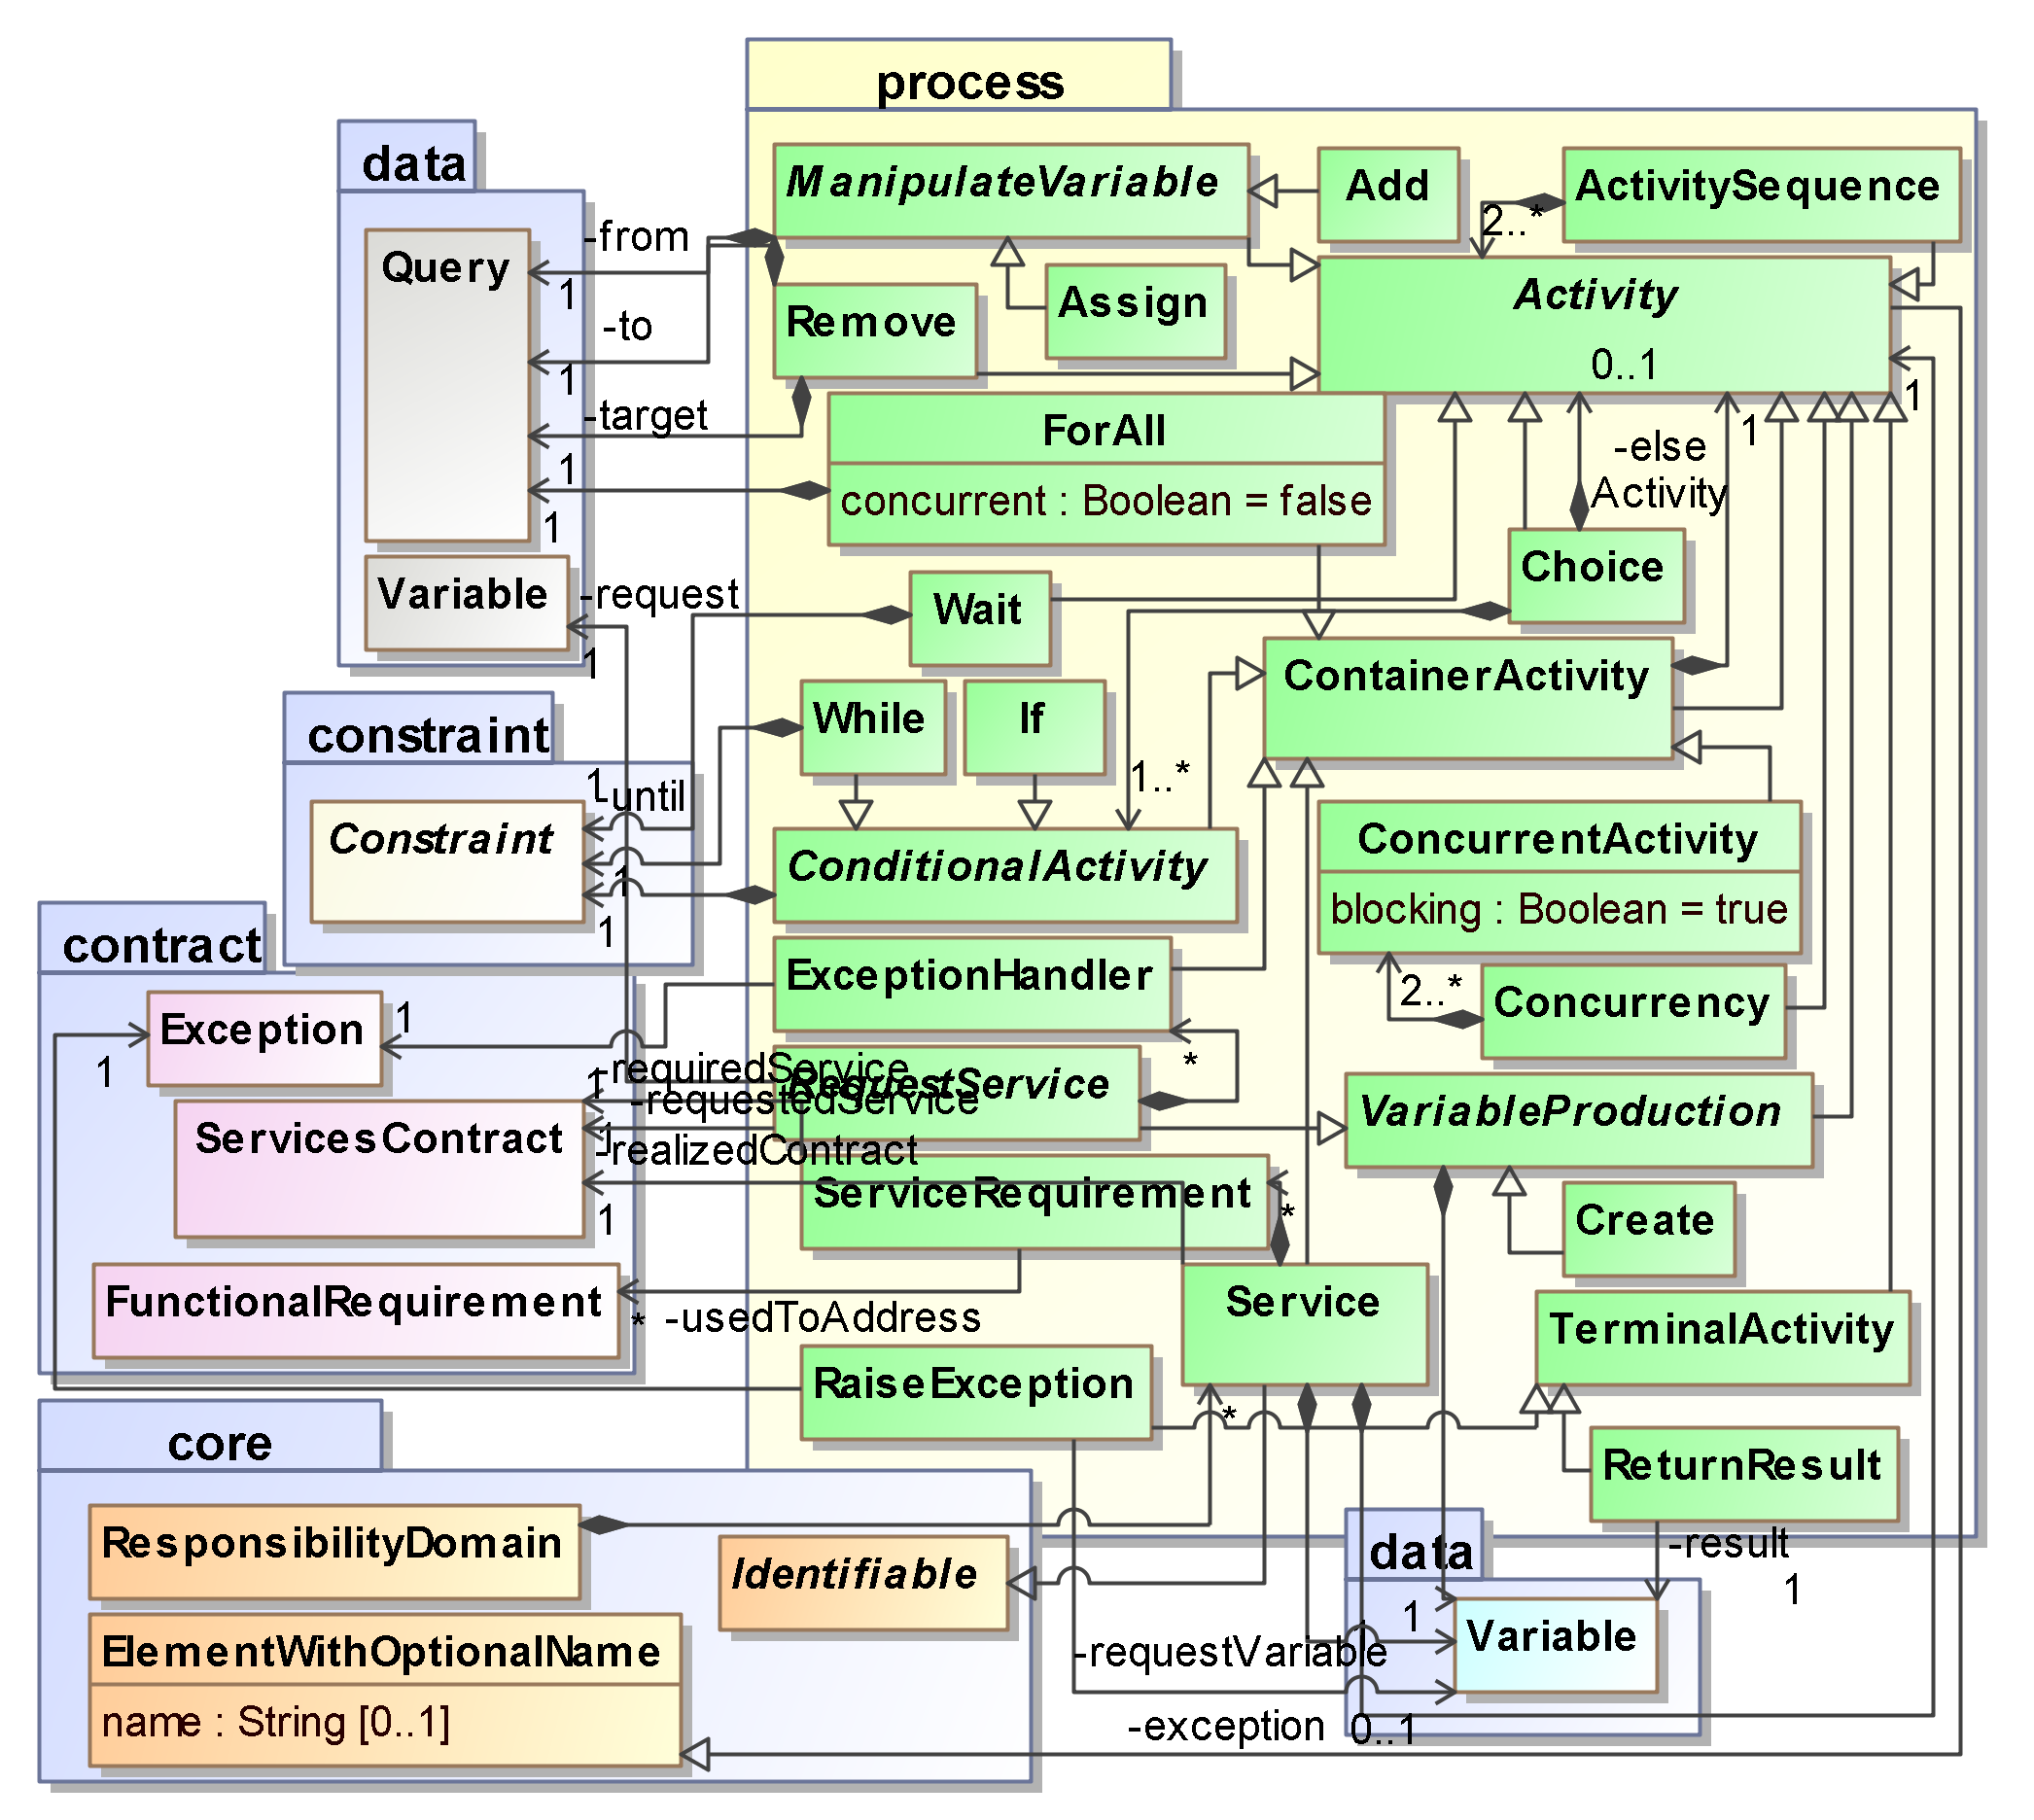
\includegraphics[width=\pagewidth]{process}\\   
  \caption{The process definition elements of URDAD}
  \label{fig:processModule}
\end{figure*}
 
